\documentclass{beamer}
% Use DS9 global theme
\usepackage{../../../shared/templates/ds9_theme}

% Title page configuration
\title[CH22 Magnetism]{PHYS12 CH22: Magnetism}
\subtitle{Sections 22.1-22.8}
\author[Mr. Gullo]{Mr. Gullo}
\date[April 2025]{April, 2025}

\begin{document}

% Title slide
\begin{frame}
\titlepage
\end{frame}

% Learning objectives
\begin{frame}{Learning Objectives}
\begin{block}{By the end of this presentation, you should be able to:}
\begin{itemize}
\item Describe magnets, magnetic fields, and magnetism
\item Understand magnetic field lines and their properties
\item Calculate the force on charges and currents in magnetic fields
\item Apply the right-hand rule for magnetic forces
\item Explain the Hall effect and practical applications
\item Calculate torque on current loops in magnetic fields
\end{itemize}
\end{block}
\end{frame}

% Outline slide
\begin{frame}{Outline}
\tableofcontents
\end{frame}

\section{Magnets and Magnetic Fields}

% Basic concepts of magnetism
\begin{frame}{Basic Concepts of Magnetism}
\begin{block}{Magnetism}
Properties of magnets and their interaction with moving charges and currents.
\end{block}

\begin{columns}
\column{0.6\textwidth}
\begin{itemize}
\item Magnetic poles: North and South
\item Like poles repel, unlike poles attract
\item Poles always occur in pairs—cannot be isolated
\item North poles point toward Earth's geographic north
\end{itemize}

\column{0.4\textwidth}
\begin{figure}
\centering
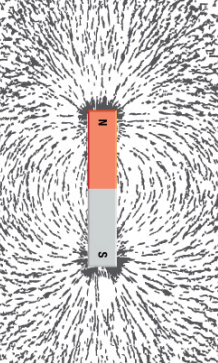
\includegraphics[width=0.8\linewidth]{phys12-magnetism-magnetic-field-generator.png}
\end{figure}
\end{columns}
\end{frame}

% Ferromagnets and Electromagnets
\begin{frame}{Ferromagnets and Electromagnets}
\begin{columns}
\column{0.5\textwidth}
\textbf{Ferromagnetic Materials}
\begin{itemize}
\item Materials with strong magnetic effects (iron)
\item Form regions called \textbf{domains}
\item Domains align to create permanent magnets
\item Lose magnetism above Curie temperature
\end{itemize}

\column{0.5\textwidth}
\textbf{Electromagnets}
\begin{itemize}
\item Use electric currents to create magnetic fields
\item Field strength depends on current and coil turns
\item Can be turned on and off
\end{itemize}
\end{columns}
\end{frame}

% Magnetic field lines
\begin{frame}{Magnetic Field Lines}
\begin{block}{Magnetic Field Representation}
Magnetic fields are represented by field lines.
\end{block}

\begin{columns}
\column{0.6\textwidth}
\textbf{Properties of magnetic field lines:}
\begin{itemize}
\item Field is tangent to the field line
\item Line density shows field strength
\item Lines never cross
\item Lines form continuous loops
\end{itemize}

\column{0.4\textwidth}
\begin{figure}
\centering
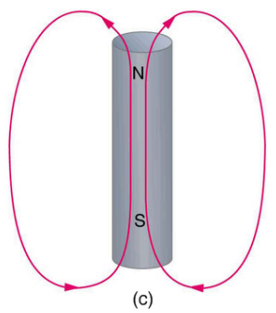
\includegraphics[width=1\linewidth]{phys12-magnetism-magnetic-force-on-wire.png}
\end{figure}
\end{columns}
\end{frame}

\section{Magnetic Forces on Charges and Currents}

% Force on moving charge
\begin{frame}{Force on Moving Charge in Magnetic Field}
\begin{block}{Magnetic Force Formula}
The magnitude of the magnetic force on a moving charge:
\begin{equation}
F = qvB\sin\theta
\end{equation}
where $\theta$ is the angle between velocity and field.
\end{block}

\begin{columns}
\column{0.5\textwidth}
\begin{itemize}
\item SI unit: tesla (T)
\item Force direction given by right-hand rule
\item Force is perpendicular to $v$ and $B$
\item No force when $v$ is parallel to $B$
\end{itemize}

\column{0.5\textwidth}
\begin{figure}
\centering
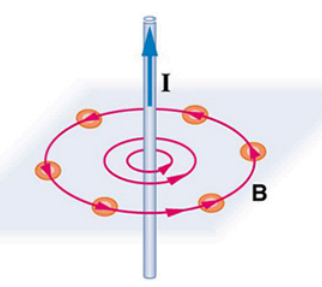
\includegraphics[width=0.75\linewidth]{phys12-magnetism-magnetic-field-lines-generator.png}
\end{figure}
\end{columns}
\end{frame}

\begin{frame}{Force on Moving Charge in Magnetic Field}
\begin{figure}
    \centering
    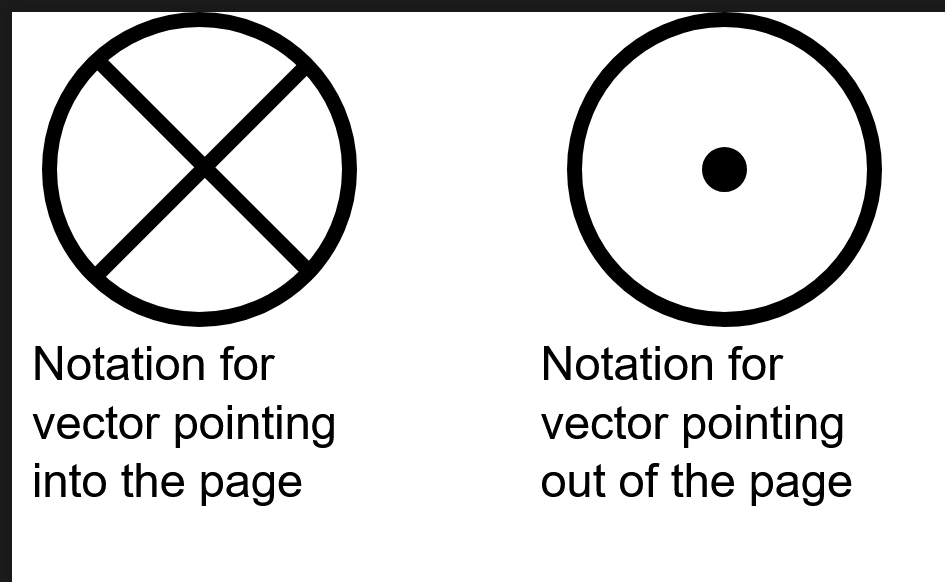
\includegraphics[width=0.75\linewidth]{phys12-vectors-vector-addition.png}
\end{figure}

\end{frame}

\begin{frame}{Force on Moving Charge in Magnetic Field}
\begin{figure}
\centering
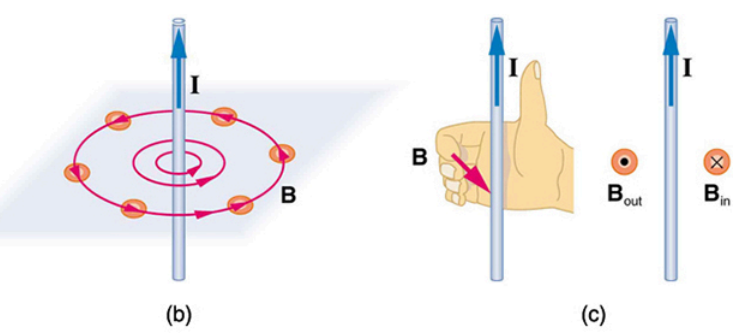
\includegraphics[width=0.75\linewidth]{phys12-magnetism-right-hand-rule-force.png}
\end{figure}
\end{frame}



\begin{frame}{Force on Moving Charge in Magnetic Field}
\begin{figure}
\centering
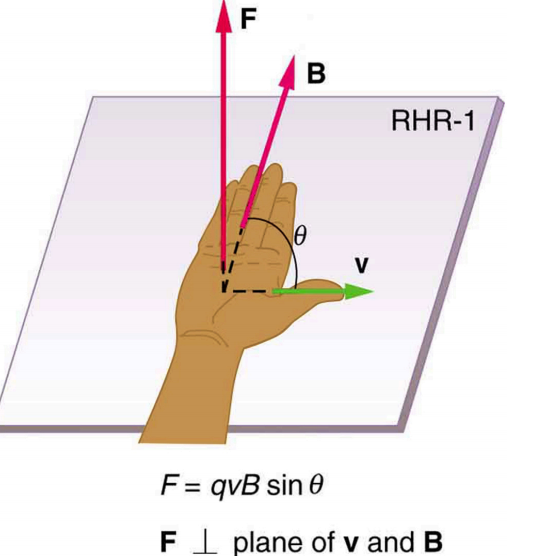
\includegraphics[width=0.8\linewidth]{phys12-magnetism-right-hand-rule-current.png}
\end{figure}
\end{frame}

% Applications of force on moving charge
\begin{frame}{Applications of Force on Moving Charges}
\begin{block}{Circular Motion in Magnetic Field}
Radius of a charged particle's circular path:
\begin{equation}
r = \frac{mv}{qB}
\end{equation}
\end{block}

\begin{columns}
\column{0.6\textwidth}
\begin{itemize}
\item Applications:
\begin{itemize}
\item Mass spectrometers
\item Particle accelerators
\item Particle detectors
\end{itemize}
\item Only affects moving charges
\end{itemize}

\column{0.4\textwidth}
\begin{figure}
\centering
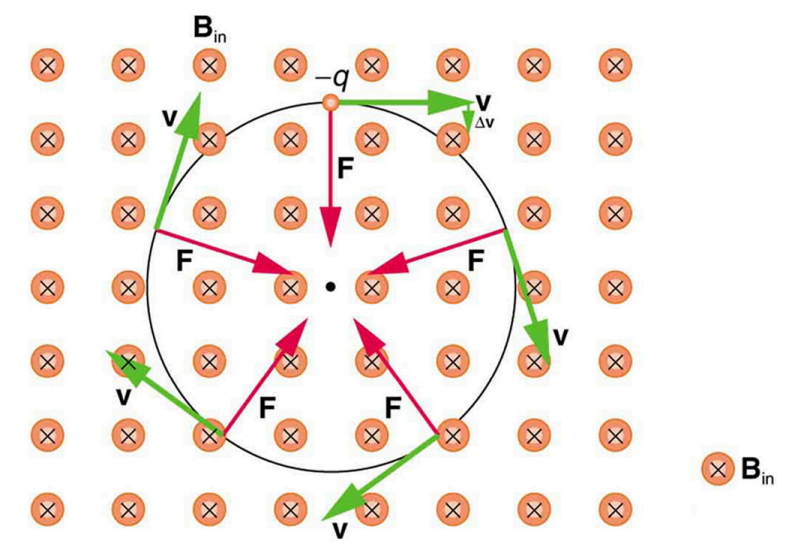
\includegraphics[width=1\linewidth]{phys12-magnetism-magnetic-force-on-current-loop.png}
\end{figure}
\end{columns}
\end{frame}

% Hall Effect
\begin{frame}{The Hall Effect}
\begin{block}{Hall Effect}
Voltage created across a current-carrying conductor by a magnetic field.
\end{block}

\begin{columns}
\column{0.5\textwidth}
\begin{itemize}
\item Hall voltage:
\begin{equation}
\varepsilon = Blv
\end{equation}
\item $B$, $l$, and $v$ must be perpendicular
\item Applications:
\begin{itemize}
\item Measuring magnetic fields
\item Hall effect sensors
\end{itemize}
\end{itemize}

\column{0.5\textwidth}
\begin{figure}
\centering
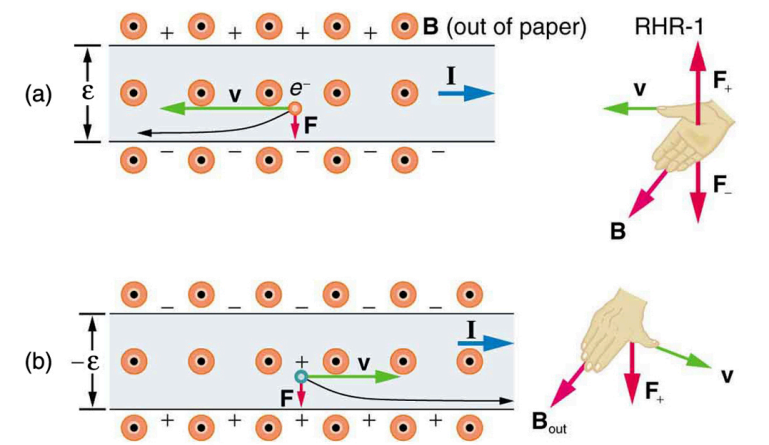
\includegraphics[width=1\linewidth]{phys12-magnetism-hall-effect.png}
\end{figure}
\end{columns}
\end{frame}

% Force on current-carrying conductor
\begin{frame}{Magnetic Force on a Current-Carrying Conductor}
\begin{block}{Force Formula}
The magnetic force on a current-carrying conductor:
\begin{equation}
F = IlB\sin\theta
\end{equation}
where $I$ is current, $l$ is length, $B$ is field strength, and $\theta$ is the angle.
\end{block}

\begin{itemize}
\item Direction follows right-hand rule
\item Maximum force when conductor is perpendicular to field
\item No force when conductor is parallel to field
\item Basis for electric motors
\end{itemize}
\end{frame}

% Torque on current loop
\begin{frame}{Torque on a Current Loop: Motors and Meters}
\begin{block}{Torque Formula}
The torque on a current-carrying loop:
\begin{equation}
\tau = NIAB\sin\theta
\end{equation}
where $N$ is turns, $I$ is current, $A$ is area, $B$ is field strength.
\end{block}

\begin{columns}
\column{0.5\textwidth}
\begin{itemize}
\item Maximum torque: loop parallel to field
\item Zero torque: loop perpendicular to field
\item Applications:
\begin{itemize}
\item Electric motors
\item Measuring instruments
\end{itemize}
\end{itemize}

\column{0.5\textwidth}
\begin{figure}
\centering
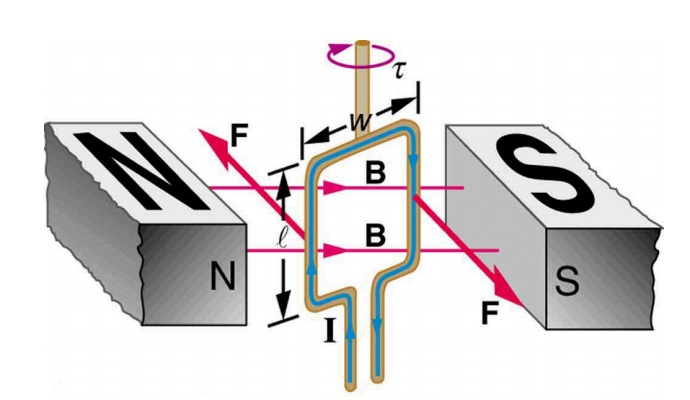
\includegraphics[width=0.9\linewidth]{phys12-magnetism-torque-on-current-loop.png}
\end{figure}
\end{columns}
\end{frame}

\section{Example Problems}

% I do example
\begin{frame}{Example 1: "I do"}
\begin{block}{Problem}
Calculate the force on an electron moving at $5.0 \times 10^6$ m/s perpendicular to a magnetic field of 0.50 T.
\end{block}
\pause
\begin{block}{Solution}
Given:
\begin{itemize}
\item Charge of electron: $-1.60 \times 10^{-19}$ C
\item Velocity: $5.0 \times 10^6$ m/s
\item Magnetic field: 0.50 T
\item Angle: $90°$ (perpendicular)
\end{itemize}
\end{block}
\end{frame}

\begin{frame}{Example 1: "I do"}
\begin{block}{Solution}
Given:
\begin{itemize}
\item Charge of electron: $-1.60 \times 10^{-19}$ C
\item Velocity: $5.0 \times 10^6$ m/s
\item Magnetic field: 0.50 T
\item Angle: $90°$ (perpendicular)
\end{itemize}

Using $F = qvB\sin\theta$:

\pause

\begin{align}
F &= (-1.60 \times 10^{-19} \text{ C})(5.0 \times 10^6 \text{ m/s})(0.50 \text{ T})(\sin 90°) \\
F &= -4.0 \times 10^{-13} \text{ N}
\end{align}

The negative sign indicates force direction opposite to the right-hand rule.
\end{block}
\end{frame}

% We do example
\begin{frame}{Example 2: "We do"}
\begin{block}{Problem}
Find the radius of the circular path of a proton with speed $3.0 \times 10^6$ m/s in a magnetic field of 0.75 T when the proton velocity is perpendicular to the field.
\end{block}
\pause

\begin{block}{Solution}
Given:
\begin{itemize}
\item Mass of proton: $1.67 \times 10^{-27}$ kg
\item Charge of proton: $1.60 \times 10^{-19}$ C
\item Velocity: $3.0 \times 10^6$ m/s
\item Magnetic field: 0.75 T
\end{itemize}
\end{block}
\end{frame}

\begin{frame}{Example 2: "We do"}
\pause
\begin{block}{Solution}
Given:
\begin{itemize}
\item Mass of proton: $1.67 \times 10^{-27}$ kg
\item Charge of proton: $1.60 \times 10^{-19}$ C
\item Velocity: $3.0 \times 10^6$ m/s
\item Magnetic field: 0.75 T
\end{itemize}

Using $r = \frac{mv}{qB}$:

\pause

\begin{align}
r &= \frac{(1.67 \times 10^{-27} \text{ kg})(3.0 \times 10^6 \text{ m/s})}{(1.60 \times 10^{-19} \text{ C})(0.75 \text{ T})} \\
r &= 4.2 \times 10^{-2} \text{ m} = 4.2 \text{ cm}
\end{align}
\end{block}
\end{frame}

% You do example
\begin{frame}{Example 3: "You do"}
\begin{block}{Problem}
A straight wire carrying a 5.0 A current is placed in a uniform magnetic field of 0.25 T. If the wire is 10 cm long and makes an angle of 30° with the field, what is the magnetic force on the wire?
\end{block}
\pause
\begin{block}{Hints}
\begin{itemize}
\item Use $F = IlB\sin\theta$
\item Convert length to meters
\item Calculate $\sin(30°)$
\end{itemize}
\end{block}
\pause
\begin{block}{Answer (to check your work)}
$F = 0.125$ N
\end{block}
\end{frame}

% Key Equations summary
\begin{frame}{Key Equations}
\begin{block}{Magnetic Forces}
\begin{align}
F &= qvB\sin\theta & \text{(Force on moving charge)} \\
r &= \frac{mv}{qB} & \text{(Radius of circular path)} \\
\varepsilon &= Blv & \text{(Hall emf)} \\
F &= IlB\sin\theta & \text{(Force on current-carrying conductor)} \\
\tau &= NIAB\sin\theta & \text{(Torque on current loop)}
\end{align}
\end{block}

\begin{block}{Right-Hand Rule}
Thumb: velocity/current direction, Fingers: magnetic field, Palm: force direction
\end{block}
\end{frame}

% Summary
\begin{frame}{Summary}
\begin{itemize}
\item Magnets have north and south poles that cannot be isolated
\item Like poles repel, unlike poles attract
\item All magnetism arises from electric current
\item Magnetic fields affect moving charges and currents
\item The Hall effect creates voltage in conductors in magnetic fields
\item Torque on current loops enables motors and meters
\end{itemize}

\begin{block}{Applications}
Electromagnets, motors, generators, particle accelerators, MRI, sensors
\end{block}
\end{frame}

% References slide
\begin{frame}{References}
\begin{block}{Textbook}
OpenStax Physics, Chapter 22: Magnetism, Sections 22.1-22.8
\end{block}
\end{frame}

\end{document}